\RequirePackage[ngerman=ngerman-x-latest]{hyphsubst}
\documentclass[aspectratio=169,xcolor={table}]{beamer}
\usetheme{metropolis}
\usepackage[T1]{fontenc}
\usepackage{selinput}
\SelectInputMappings{adieresis={ä},germandbls={ß}}
\usepackage[defaultsans]{opensans}
\usepackage[table]{xcolor}
\usepackage{pifont}
\usepackage{float}
\usepackage{amsmath}
\usepackage{appendixnumberbeamer}
\usepackage{url}
\usepackage{adjustbox}
\usepackage{tikz}
\usetikzlibrary{arrows,arrows.meta}
\usepackage{threeparttable}
\usepackage{wasysym}
\usepackage{xstring}
\usepackage{amsthm}
\usepackage{caption}
\usepackage{graphicx}
\usepackage{array}
\usepackage{booktabs}
\newcommand*\rot{\bfseries\rotatebox{90}}
\usepackage{subcaption}
\usepackage{listings}
\lstloadlanguages{Prolog}
\usepackage{pdfpages}
\usepackage{babel}
\usepackage{csquotes}
\usepackage{graphicx}
\usepackage{import}
\usepackage{microtype}
\usepackage[backend=biber,style=authoryear, maxcitenames=1]{biblatex}
\DefineBibliographyStrings{ngerman}{andothers={et\ al\adddot}} 
\AtEveryCite{%
  \let\parentext=\parentexttrack%
  \let\bibopenparen=\bibopenbracket%
  \let\bibcloseparen=\bibclosebracket}
\addbibresource{sources.bib}
\usepackage{hyperref}
\usepackage[noabbrev]{cleveref}

%\counterwithout{figure}{chapter}
%\counterwithout{equation}{chapter}

\newcommand{\cmark}{\ding{51}}%
\newcommand{\xmark}{\ding{55}}%

\newcommand{\f}[1]{%
    \IfEqCase{#1}{%
        {H}{\CIRCLE}%
        {M}{\LEFTcircle}%
        {L}{\Circle}%
        {0}{\xmark}%
        {1}{\cmark}%
    }[\PackageError{f}{Undefined option to f: #1}{}]%
}%

\lstset{
  basicstyle=\footnotesize, 
  frame=tb,
  xleftmargin=.05\textwidth, 
  xrightmargin=.05\textwidth,
  aboveskip=16pt, belowskip=16pt,
  captionpos=b,
  numbers=left,
  numberbychapter=false,
  extendedchars=true,
  literate={ä}{{\"a}}1 {ö}{{\"o}}1 {ü}{{\"u}}1 {Ä}{{\"A}}1 {Ö}{{\"O}}1 {Ü}{{\"U}}1,
}

\lstdefinelanguage{Kotlin}{
  comment=[l]{//},
  emph={delegate, filter, first, firstOrNull, forEach, lazy, map, mapNotNull, println, return@},
  keywords={abstract, actual, as, as?, break, by, class, companion, continue, data, do, dynamic, else, enum, expect, false, final, for, fun, get, if, import, in, interface, internal, is, null, object, override, package, private, public, return, set, super, suspend, this, throw, true, try, typealias, val, var, vararg, when, where, while},
  morecomment=[s]{/*}{*/},
  morestring=[b]",
  morestring=[s]{"""*}{*"""},
  ndkeywords={@Deprecated, @JvmField, @JvmName, @JvmOverloads, @JvmStatic, @JvmSynthetic, Array, Byte, Double, Float, Int, Integer, Iterable, Long, Runnable, Short, String},
  sensitive=true,
}

\crefname{listing}{Quelltext}{Quelltext}
\Crefname{listing}{Quelltext}{Quelltext}

\definecolor{layer1}{HTML}{000000}
\definecolor{layer2}{HTML}{2196F3}
\definecolor{layer3}{HTML}{689F38}
\definecolor{rowhighlight}{HTML}{e8e8e8}
\definecolor{unimportant}{HTML}{bababa}
\definecolor{background}{HTML}{fafafa}
\definecolor{error}{HTML}{f44336}

\tikzset{%
    >={Latex[length=3mm]}
}
\newcommand\MMElement[5]{%
    \draw (#1-#3/2,#2-#4/2) rectangle (#1+#3/2,#2+#4/2);
    \draw (#1,#2) node {#5}
}

\title{\phantom{\small x}\\\textnormal{\small Verteidigung Bachelorarbeit}\\Evaluierung der Konsistenz zwischen Business Process Modellen und Business Role-Object Spezifikation}
\author{Lars Westermann}
\date{26.09.2019}
\institute{
  Institut für Software- und Multimediatechnik, Professur für Softwaretechnologie\\\\
  Prof. Dr. rer. nat. habil. Uwe Aßmann\\
  Dr.-Ing. Thomas Küh\\
  Hendrik Schön\\
}

%\advisor{Hendrik Schön}
%\supervisor{Dr.-Ing. Thomas Kühn}
%\professor{Prof. Dr. rer. nat. habil. Uwe Aßmann}

\begin{document}
  \maketitle

  \begin{frame}{Motivation}
  Diskrepanz zwischen Modellierungaspekten:

  \begin{itemize}
    \item \textbf{Strukturmodellierung} mittels z.B. UML-Klassen- oder Komponentendiagrammen 

    \item \textbf{Verhaltensmodellierung} mittels z.B. UML-Sequenzdiagrammen oder Petrinetzen
  \end{itemize}
\end{frame}
\begin{frame}{Motivation}
  \begin{figure}
  \centering
  \begin{adjustbox}{width=.75\linewidth,center}
    \begin{tikzpicture}
      \draw[dashed] (0,4.7) -- (0,-5.2);

      \begin{scope}[shift={(0,-0.25)}]
        \draw (-8,2.5) rectangle (-1,-2.5);
        \draw (-8,1.5) -- (-1,1.5);
        \draw (-8,0.5) -- (-1,0.5);
        \draw (-4.5,2) node{Chef};
        \draw (-8,-0.2) node[anchor=west] {passOrder(order: Order): Bool};
        \draw (-8,-1) node[anchor=west] {isOrderFinished(order: Order): Bool};
        \draw (-8,-1.8) node[anchor=west] {getPizza(order: Order): Pizza};
      \end{scope}

      \draw (4, 4.2) circle[radius=0.5];
      \draw[->] (4,3.7) -- (4,2.5);
      \draw (4,3.1) node[anchor=west] {passOrder(x)};
      \draw[rounded corners=4.8pt] (1,2.5) rectangle (7,1.5);
      \draw (4,2) node {Order in processing};
      \draw[->] (4,1.5) -- (4,0.5);
      \draw (4,0.5) -- (4.5,0) -- (4,-0.5) -- (3.5,0) -- cycle;
      \draw[->] (4.5,0) -- (8,0)-- (8,2) -- (7,2);
      \draw (4.7,-0.2) -- (4.8,0.2);
      \draw[->] (4,-0.5) -- (4,-2);
      \draw (4,-0.9) node[anchor=west] {checkOrderState(x) ==};
      \draw (5.5,-1) node[anchor=north west] {State.FINISHED};
      \draw[rounded corners=4.8pt] (1,-3) rectangle (7,-2);
      \draw (4,-2.5) node {Order ready for serving};
      \draw[->] (4,-3) -- (4,-4.2);
      \draw (4,-3.6) node[anchor=west] {getPizza(x)};
      \draw (4, -4.7) circle[radius=0.5];
      \fill (4, -4.7) circle[radius=0.3];

      \draw[dashed,color=layer3,line width=0.025cm] (-1,-0.45) -- (0.5,-0.45) -- (0.5,3.1) -- (4,3.1);
      \draw[dashed,color=layer3,line width=0.025cm] (-1,-1.25) -- (1,-1.25) -- (1,-1.1) -- (4,-1.1);
      \draw[dashed,color=layer3,line width=0.025cm] (-1,-2.05) -- (0.5,-2.05) -- (0.5,-3.6) -- (4,-3.6);
    \end{tikzpicture}
  \end{adjustbox}
\end{figure}

\end{frame}

\begin{frame}{Problemdefinition}
  Es gibt viele Verfahren zur Konsistenzprüfung bestehenden Struktur- und Verhaltensmodellierungsprachen

  Dies gilt nicht für die Konsistenz zwischen \textbf{BPMN} und \textbf{BROS}:

  \begin{itemize}
    \item Es existieren noch keine Konsistenzbeziehungen

    \item Damit auch kein automatisierbares Verfahren zur Konsistenzprüfung
  \end{itemize}
\end{frame}

\begin{frame}{Forschungsfragen}
  \begin{description}[4cm]
    \item[F1] Welche Konsistenzbeziehungen bestehen zwischen BPMN- und BROS-Modellen?

    \item[F2] Wie lassen sich die Konsistenzbedingungen automatisiert überprüfen?

    \item[F3] Mit welchem Aufwand ist dieses Verfahren erweiterbar?
  \end{description}
\end{frame}

  \section{Welche Konsistenzbeziehungen bestehen zwischen BPMN- und BROS-Modellen?}

\begin{frame}{Konsistenzproblem}

  Die \textbf{Konsistenz}: Zusammenhang, Widerspruchsfreiheit [\cite{duden}]

  Eine \textbf{Inkonsistenz} tritt genau dann auf, wenn eine Konsistenzregel verletzt wird. [\cite{Nuseibeh1996}]

  Eine \textbf{Konsistenzregel} ist eine Formalisierung von einem Aspekt der Konsistenz zwischen den betrachteten Modellen. [vgl. \cite{Nuseibeh1996}]

  Das \textbf{Konsistenzproblem} beschreibt den Vorgang der Minimierung und Verhinderung von Inkonsistenzen mit Hilfe der Aufstellung und Prüfung von Konsistenzregeln.
\end{frame}

\begin{frame}{Business Process Model and Notation\footnote{\url{https://www.omg.org/spec/BPMN/2.0/About-BPMN/}}}
  \vspace{8pt}
  \begin{figure}
    \centering
    \begin{adjustbox}{width=1.1\linewidth,center}
      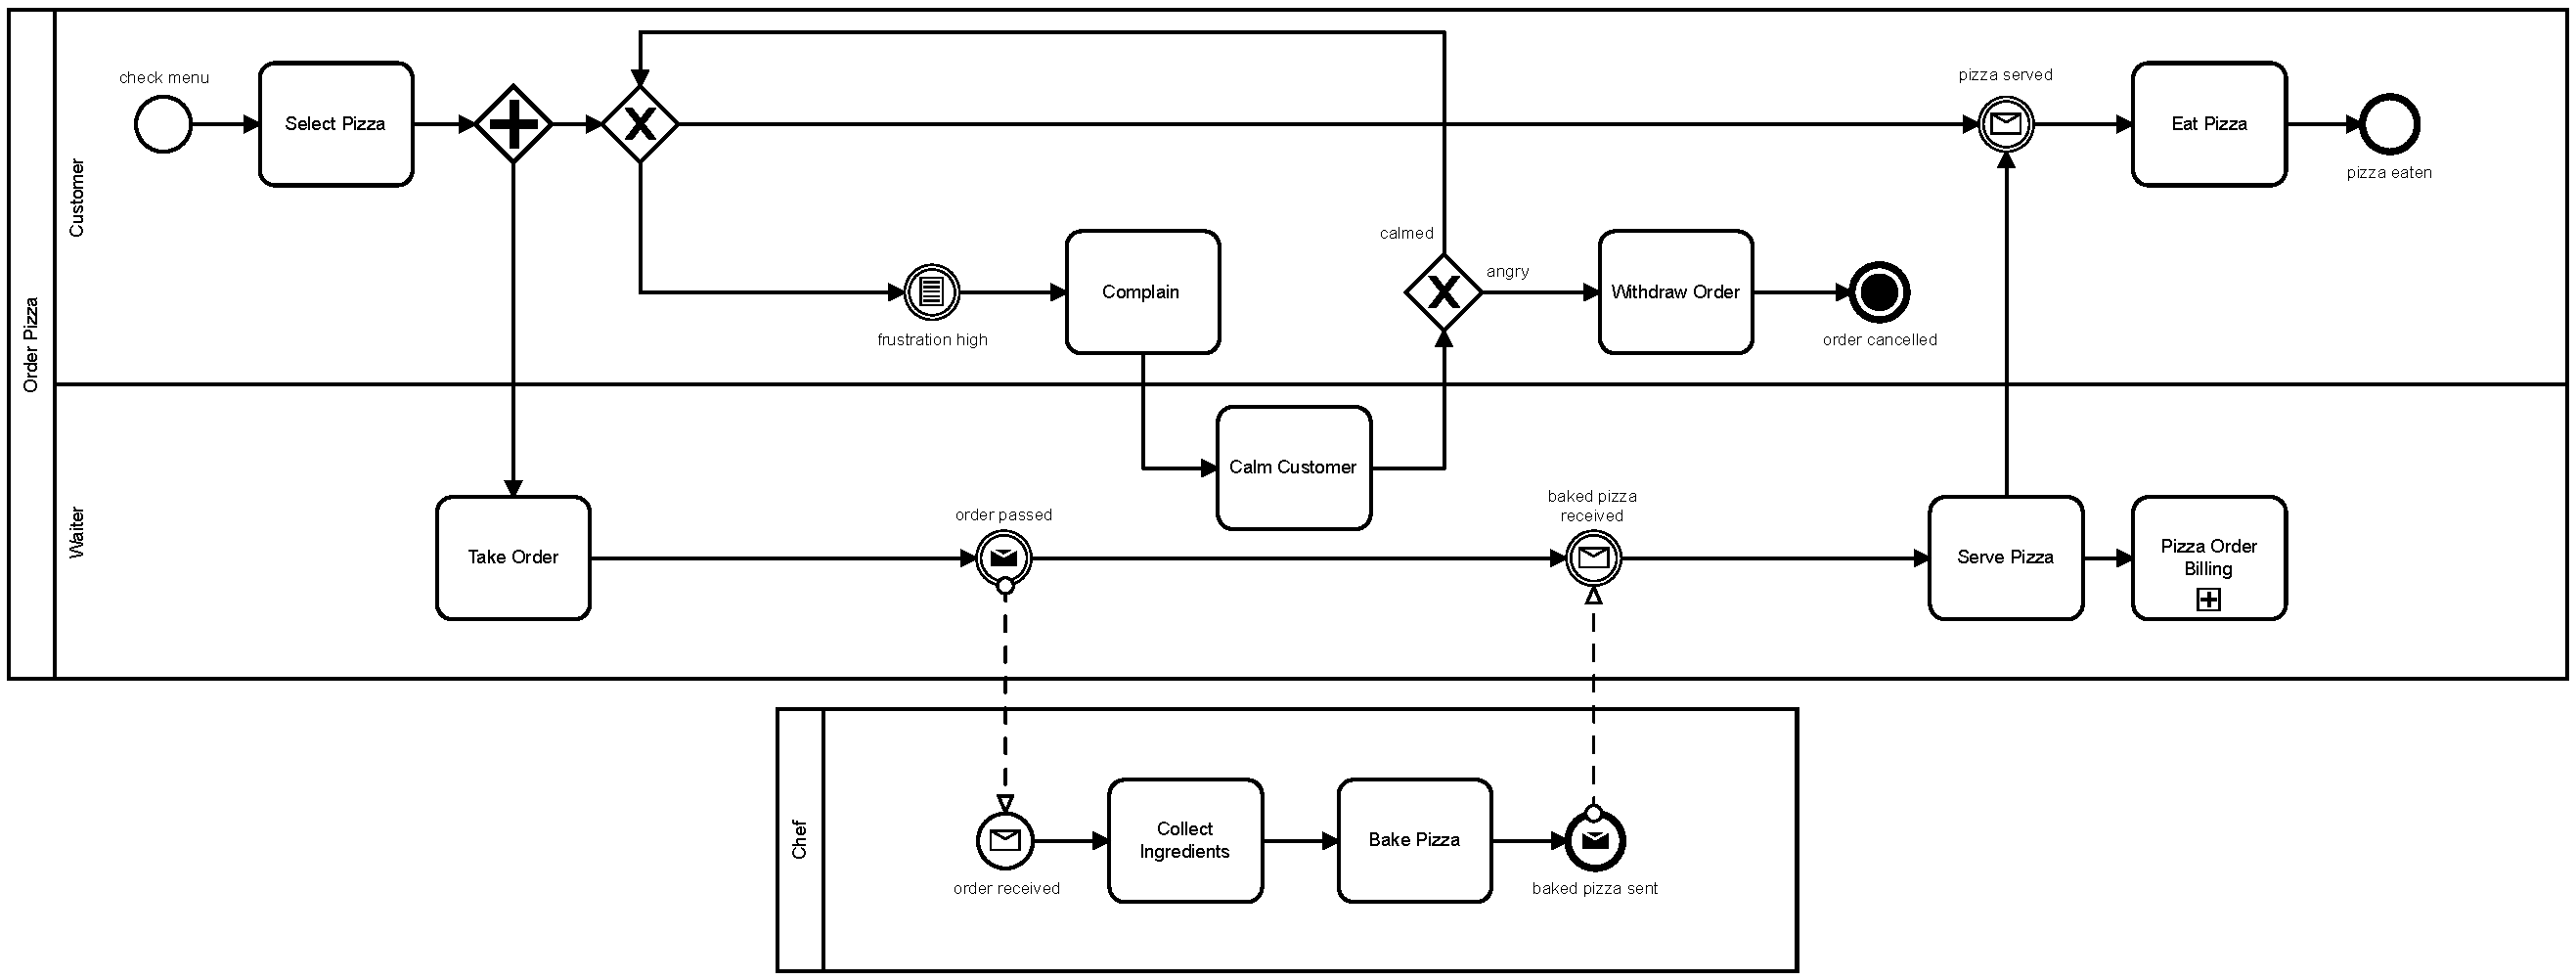
\includegraphics{images/example/bpmn.pdf}
    \end{adjustbox}
  \end{figure}
  \vspace{18.5pt}
\end{frame}
\begin{frame}{Business Role-Object Specification\footnote{\cite{Schoen}}}
  \begin{figure}
    \centering
    \begin{adjustbox}{width=0.9\linewidth,center}
      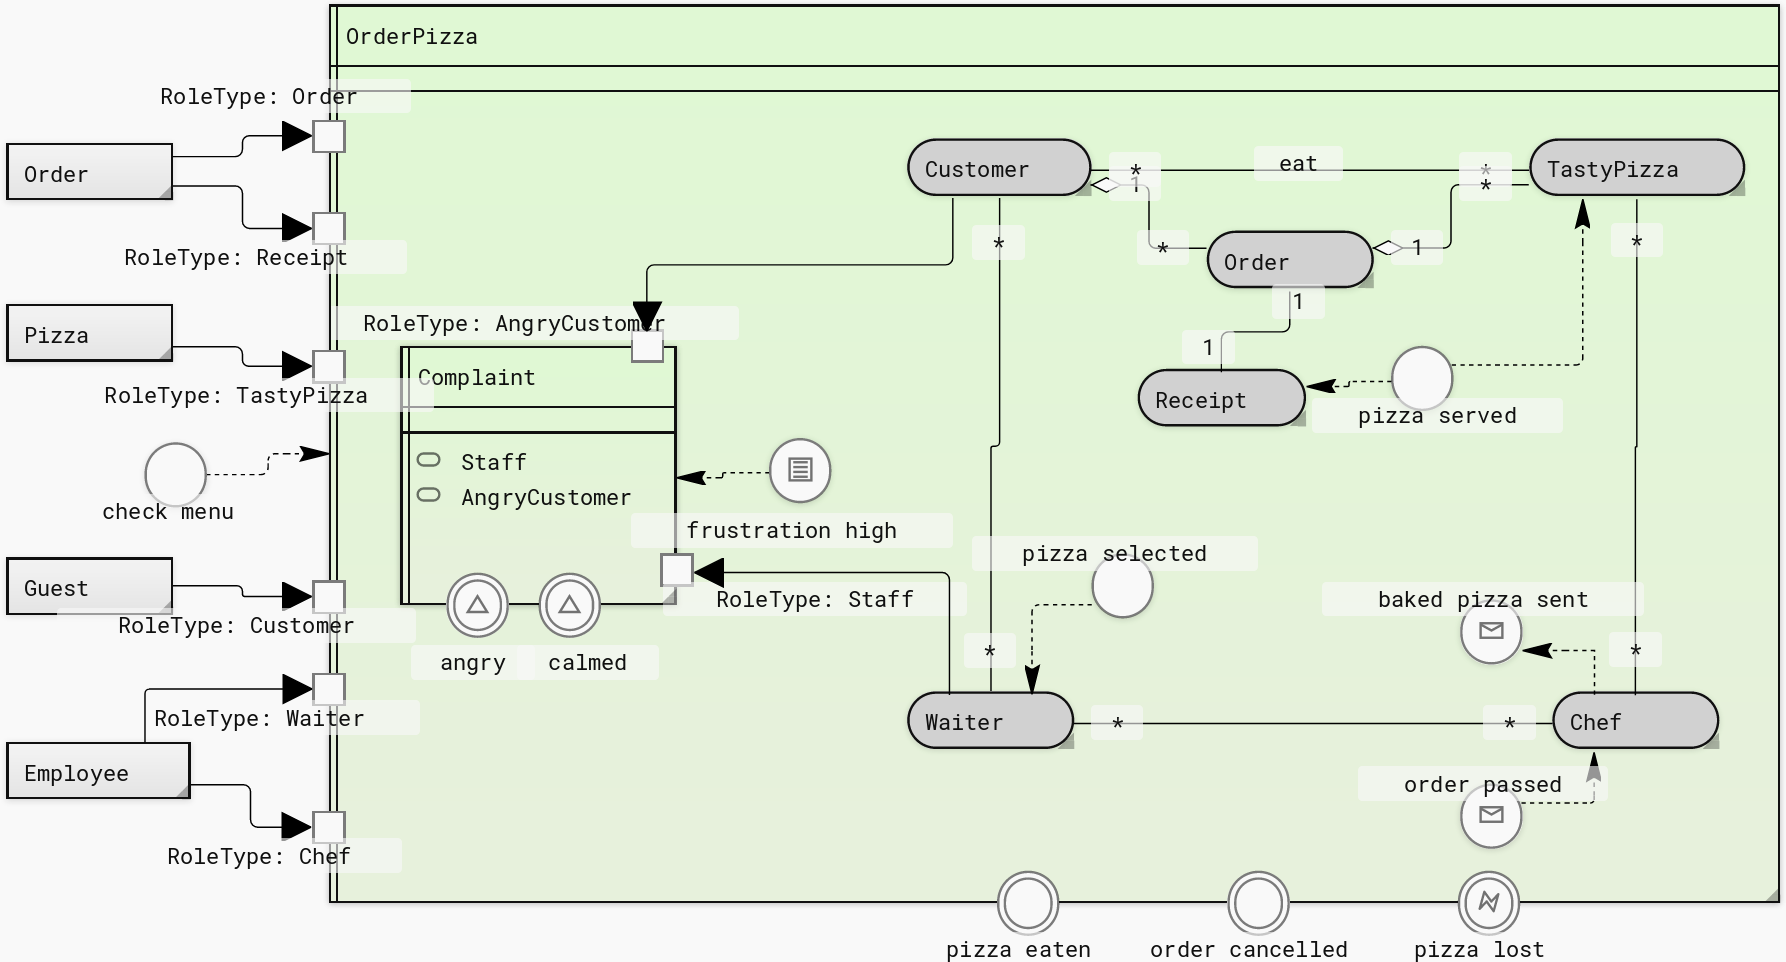
\includegraphics{images/example/bros-rule6.png}
    \end{adjustbox}
  \end{figure}
\end{frame}

\begin{frame}[fragile]{Prolog-Datenstrukutr}
\begin{lstlisting}[language=Prolog]
% Definition aller BPMN Elemente.
bpmn(Bpmn, Type).

% Definition aller BROS Elemente.
bros(Bros, Type).

% Definition aller Relationen.
relation(Source, Target, Type).

% Definition der Eltern-Kind Beziehung.
parent(Child, Parent).
\end{lstlisting}
\end{frame}
\begin{frame}[fragile]{Hilfsfunktionen}
\begin{lstlisting}[language=Prolog]
% Konsistenz der Eltern-Kind Beziehung.
check_parent(C) :- 
  parent(C, P), parent(C, Q) -> P == Q.

% Transitiver Abschluss der Modellstruktur (gekürzt).
transitive_parent(Child, Parent).

% Orakel für das Matching von Modellelementen.
match(Bpmn, Bros).
\end{lstlisting}
\end{frame}

\begin{frame}{Konsistenzbeziehungen}
  \begin{figure}
    \centering
    \begin{subfigure}{0.3\textwidth}
        \centering
        \begin{adjustbox}{width=0.8\linewidth,center}
          \begin{tikzpicture}
            \node at (0,0) {\begin{tikzpicture}[scale=0.5, every node/.style={scale=0.8},>={Latex[length=1.5mm]}]
  \draw[dashed] (-8,-7) -- (8,7);
  \draw (-6,-5.25) node[anchor=south, rotate=41] {\textbf{BPMN}};
  \draw (-6,-5.25) node[anchor=north, rotate=41] {BROS};

  \draw (-8,6) rectangle (0,1);
  \draw (-7,6) -- (-7,1);
  \draw (-7.5,3.5) node[rotate=90] {Order Pizza};
  \draw (-7,3.5) -- (0,3.5);
  \draw (-6.5,4.75) node[color=unimportant,rotate=90] {A};
  \draw (-6.5,2.25) node[color=unimportant,rotate=90] {B};

  \draw[rounded corners=4.8pt] (0,-0.5) rectangle (8,-6.5);
  \draw (0.2,-0.56) -- (0.2,-6.44);
  \draw (0,-1.5) -- (8,-1.5);
  \draw (4,-1) node {OrderPizza};

  \begin{scope}[color=unimportant]
      \draw[rounded corners=4.8pt] (4.2,-2) rectangle (7.2,-4);
      \draw (4.2,-3) -- (7.2,-3);
      \draw (4.2,-3.5) -- (7.2,-3.5);
      \draw (5.6,-2.5) node {A};

      \draw[rounded corners=4.8pt] (0.8,-4) rectangle (3.8,-6);
      \draw (0.8,-5) -- (3.8,-5);
      \draw (0.8,-5.5) -- (3.8,-5.5);
      \draw (2.4,-4.5) node {B};
  \end{scope}
\end{tikzpicture}
};
            \filldraw[draw=background,fill=background,fill opacity=0, draw opacity=0] (-4,-3.5) rectangle (4,3.5);
          \end{tikzpicture}
        \end{adjustbox}
        \caption*{\tiny{Regel 1: BPMN-Process}}%
    \end{subfigure}
    \hfill
    \begin{subfigure}{0.3\textwidth}
        \centering
        \begin{adjustbox}{width=0.8\linewidth,center}
          \begin{tikzpicture}
            \node at (0,0) {\begin{tikzpicture}[scale=0.5, every node/.style={scale=0.8},>={Latex[length=1.5mm]}]
  \draw[dashed] (-8,-7) -- (8,7);
  \draw (-6,-5.25) node[anchor=south, rotate=41] {\textbf{BPMN}};
  \draw (-6,-5.25) node[anchor=north, rotate=41] {BROS};

  \draw (-8,6) rectangle (0,1);
  \draw (-7,6) -- (-7,1);
  \draw (-7.5,3.5) node[rotate=90] {Chef};

  \draw[rounded corners=4.8pt,color=unimportant] (0,-0.5) rectangle (8,-6.5);
  \draw[color=unimportant] (0.2,-0.56) -- (0.2,-6.44);
  \draw[color=unimportant] (0,-1.5) -- (8,-1.5);
  \draw[color=unimportant] (4,-1) node {OrderPizza};

  \draw[rounded corners=4.8pt] (2.5,-3) rectangle (5.5,-5);
  \draw (2.5,-4) -- (5.5,-4);
  \draw (2.5,-4.5) -- (5.5,-4.5);
  \draw (4,-3.5) node {Chef};
\end{tikzpicture}
};
            \filldraw[draw=background,fill=background,fill opacity=0, draw opacity=0] (-4,-3.5) rectangle (4,3.5);
          \end{tikzpicture}
        \end{adjustbox}
        \caption*{\tiny{Regel 2: BPMN-Swimlane}}%
    \end{subfigure}
    \hfill
    \begin{subfigure}{0.3\textwidth}
        \centering
        \begin{adjustbox}{width=0.8\linewidth,center}
          \begin{tikzpicture}
            \node at (0,0) {\begin{tikzpicture}[scale=0.5, every node/.style={scale=0.8},>={Latex[length=1.5mm]}]
  \draw[dashed] (-8,-7) -- (8,7);
  \draw (-6,-5.25) node[anchor=south, rotate=41] {\textbf{BPMN}};
  \draw (-6,-5.25) node[anchor=north, rotate=41] {BROS};

  \draw (-8,6) rectangle (0,1);
  \draw (-7,6) -- (-7,1);
  \draw (-7.5,3.5) node[rotate=90] {Order Pizza};
  \draw (-6.5,4.5) node[rotate=90] {A};
  \draw (-6.5,2) node[rotate=90] {B};
  \draw (-7,3) -- (0,3);

  \begin{scope}[color=unimportant]
      \draw (-5,4.5) circle[radius=0.5];
      \draw (-5,4) node[anchor=north] {Start};
      \draw[->] (-4.5,4.5) -- (-2,4.5);
  \end{scope}
  \fill (-1.5,4.5) circle[radius=0.5];
  \fill[color=background] (-1.5,4.5) circle[radius=0.35];
  \fill (-1.5,4.5) circle[radius=0.2];
  \draw (-1.5,4) node[anchor=north] {End};

  \draw[rounded corners=4.8pt] (0,-0.5) rectangle (8,-6.5);
  \draw (0.2,-0.56) -- (0.2,-6.44);
  \draw (0,-1.5) -- (8,-1.5);
  \draw (4,-1) node {OrderPizza};

  \begin{scope}[color=unimportant]
      \draw[rounded corners=4.8pt] (4.2,-2) rectangle (7.2,-4);
      \draw (4.2,-3) -- (7.2,-3);
      \draw (4.2,-3.5) -- (7.2,-3.5);
      \draw (5.6,-2.5) node {A};

      \draw[rounded corners=4.8pt] (0.8,-4) rectangle (3.8,-6);
      \draw (0.8,-5) -- (3.8,-5);
      \draw (0.8,-5.5) -- (3.8,-5.5);
      \draw (2.4,-4.5) node {B};
  \end{scope}

  \filldraw[fill=background] (0,-4) circle[radius=0.5];
  \draw (0,-4) circle[radius=0.35];
  \draw (0,-4.5) node[anchor=north,fill=background] {End};
\end{tikzpicture}
};
            \filldraw[draw=background,fill=background,fill opacity=0, draw opacity=0] (-4,-3.5) rectangle (4,3.5);
          \end{tikzpicture}
        \end{adjustbox}
        \caption*{\tiny{Regel 3: BPMN-TerminationEvent}}%
    \end{subfigure}
    \begin{subfigure}{0.3\textwidth}
        \vspace{4pt}
        \centering
        \begin{adjustbox}{width=0.8\linewidth,center}
          \begin{tikzpicture}
            \node at (0,0) {\begin{tikzpicture}[scale=0.5, every node/.style={scale=0.8},>={Latex[length=1.5mm]}]
  \draw[dashed] (-8,-7) -- (8,7);
  \draw (-6,-5.25) node[anchor=south, rotate=41] {\textbf{BPMN}};
  \draw (-6,-5.25) node[anchor=north, rotate=41] {BROS};

  \draw (-8,6) rectangle (0,1);
  \draw (-7,6) -- (-7,1);
  \draw (-7.5,3.5) node[rotate=90] {Chef};

  \begin{scope}[color=unimportant]
      \draw (-5.5,3.5) circle[radius=0.5];
      \draw (-5.5,3) node[anchor=north] {Start};
      \draw[->] (-5,3.5) -- (-2,3.5);
  \end{scope}
  \fill (-1.5,3.5) circle[radius=0.5];
  \fill[color=white] (-1.5,3.5) circle[radius=0.35];
  \draw (-1.5,3) node[anchor=north] {End};

  \draw[rounded corners=4.8pt] (0,-0.5) rectangle (8,-6.5);
  \draw (0.2,-0.56) -- (0.2,-6.44);
  \draw (0,-1.5) -- (8,-1.5);
  \draw (4,-1) node {OrderPizza};

  \draw[rounded corners=4.8pt] (4,-3) rectangle (7,-5);
  \draw (4,-4) -- (7,-4);
  \draw (4,-4.5) -- (7,-4.5);
  \draw (5.5,-3.5) node {Chef};

  \begin{scope}[color=unimportant]
      \draw (1.5,-2.5) circle[radius=0.5];
      \draw (1.5,-3) node[anchor=north] {Start};
      \draw[dashed, ->] (2,-2.5) -- (5.5,-2.5) -- (5.5,-3);
  \end{scope}

  \draw (1.5,-5.5) circle[radius=0.5];
  \draw (1.5,-6) node[anchor=north,fill=white] {End};
  \draw[dashed, ->] (5.5,-5) -- (5.5,-5.5) -- (2,-5.5);
\end{tikzpicture}
};
            \filldraw[draw=background,fill=background,fill opacity=0, draw opacity=0] (-4,-3.5) rectangle (4,3.5);
          \end{tikzpicture}
        \end{adjustbox}
        \caption*{\tiny{Regel 4: BPMN-EndEvent}}%
    \end{subfigure}
    \hspace{16pt}
    \begin{subfigure}{0.3\textwidth}
        \vspace{4pt}
        \centering
        \begin{adjustbox}{width=0.8\linewidth,center}
          \begin{tikzpicture}
            \node at (0,0) {\begin{tikzpicture}[scale=0.5, every node/.style={scale=0.8},>={Latex[length=1.5mm]}]
  \draw[dashed] (-8,-7) -- (8,7);
  \draw (-6,-5.25) node[anchor=south, rotate=41] {\textbf{BPMN}};
  \draw (-6,-5.25) node[anchor=north, rotate=41] {BROS};

  \draw (-8,6) rectangle (0,1);
  \draw (-7,6) -- (-7,1);
  \draw (-7.5,3.5) node[rotate=90] {Chef};

  \draw (-5.5,3.5) circle[radius=0.5];
  \draw (-5.5,3) node[anchor=north] {Start};
  \begin{scope}[color=unimportant]
      \draw[->] (-5,3.5) -- (-2,3.5);
      \fill (-1.5,3.5) circle[radius=0.5];
      \fill[color=background] (-1.5,3.5) circle[radius=0.35];
      \draw (-1.5,3) node[anchor=north] {End};
  \end{scope}

  \draw[rounded corners=4.8pt] (0,-0.5) rectangle (8,-6.5);
  \draw (0.2,-0.56) -- (0.2,-6.44);
  \draw (0,-1.5) -- (8,-1.5);
  \draw (4,-1) node {OrderPizza};

  \draw[rounded corners=4.8pt] (4,-3) rectangle (7,-5);
  \draw (4,-4) -- (7,-4);
  \draw (4,-4.5) -- (7,-4.5);
  \draw (5.5,-3.5) node {Chef};

  \draw (1.5,-2.5) circle[radius=0.5];
  \draw (1.5,-3) node[anchor=north] {Start};
  \draw[dashed, ->] (2,-2.5) -- (5.5,-2.5) -- (5.5,-3);

  \begin{scope}[color=unimportant]
      \draw (1.5,-5.5) circle[radius=0.5];
      \draw (1.5,-6) node[anchor=north,fill=background] {End};
      \draw[dashed, ->] (5.5,-5) -- (5.5,-5.5) -- (2,-5.5);
  \end{scope}
\end{tikzpicture}
};
            \filldraw[draw=background,fill=background,fill opacity=0, draw opacity=0] (-4,-3.5) rectangle (4,3.5);
          \end{tikzpicture}
        \end{adjustbox}
        \caption*{\tiny{Regel 5: BPMN-StartEvent}}%
    \end{subfigure}
  \end{figure}
\end{frame}

\begin{frame}{Konsistenzbeziehungen}
  \begin{figure}
    \centering
    \begin{subfigure}{0.3\textwidth}
        \centering
        \begin{adjustbox}{width=0.8\linewidth,center}
          \begin{tikzpicture}
            \node at (0,0) {\begin{tikzpicture}[scale=0.5, every node/.style={scale=0.8},>={Latex[length=1.5mm]}]
  \draw[dashed] (-8,-7) -- (8,7);
  \draw (-6,-5.25) node[anchor=south, rotate=41] {\textbf{BPMN}};
  \draw (-6,-5.25) node[anchor=north, rotate=41] {BROS};

  \draw (-8,6) rectangle (0,1);
  \draw (-7,6) -- (-7,1);
  \draw (-7.5,3.5) node[rotate=90] {Order Pizza};
  \draw (-7,3.5) -- (0,3.5);
  \draw (-6.5,4.75) node[color=unimportant,rotate=90] {A};
  \draw (-6.5,2.25) node[color=unimportant,rotate=90] {B};

  \draw[rounded corners=4.8pt] (0,-0.5) rectangle (8,-6.5);
  \draw (0.2,-0.56) -- (0.2,-6.44);
  \draw (0,-1.5) -- (8,-1.5);
  \draw (4,-1) node {OrderPizza};

  \begin{scope}[color=unimportant]
      \draw[rounded corners=4.8pt] (4.2,-2) rectangle (7.2,-4);
      \draw (4.2,-3) -- (7.2,-3);
      \draw (4.2,-3.5) -- (7.2,-3.5);
      \draw (5.6,-2.5) node {A};

      \draw[rounded corners=4.8pt] (0.8,-4) rectangle (3.8,-6);
      \draw (0.8,-5) -- (3.8,-5);
      \draw (0.8,-5.5) -- (3.8,-5.5);
      \draw (2.4,-4.5) node {B};
  \end{scope}
\end{tikzpicture}
};
            \filldraw[draw=background,fill=background,fill opacity=0.8, draw opacity=0.8] (-4,-3.5) rectangle (4,3.5);
          \end{tikzpicture}
        \end{adjustbox}
        \caption*{\tiny{\textcolor{black!20}{Regel 1: BPMN-Process}}}%
    \end{subfigure}
    \hfill
    \begin{subfigure}{0.3\textwidth}
        \centering
        \begin{adjustbox}{width=0.8\linewidth,center}
          \begin{tikzpicture}
            \node at (0,0) {\begin{tikzpicture}[scale=0.5, every node/.style={scale=0.8},>={Latex[length=1.5mm]}]
  \draw[dashed] (-8,-7) -- (8,7);
  \draw (-6,-5.25) node[anchor=south, rotate=41] {\textbf{BPMN}};
  \draw (-6,-5.25) node[anchor=north, rotate=41] {BROS};

  \draw (-8,6) rectangle (0,1);
  \draw (-7,6) -- (-7,1);
  \draw (-7.5,3.5) node[rotate=90] {Chef};

  \draw[rounded corners=4.8pt,color=unimportant] (0,-0.5) rectangle (8,-6.5);
  \draw[color=unimportant] (0.2,-0.56) -- (0.2,-6.44);
  \draw[color=unimportant] (0,-1.5) -- (8,-1.5);
  \draw[color=unimportant] (4,-1) node {OrderPizza};

  \draw[rounded corners=4.8pt] (2.5,-3) rectangle (5.5,-5);
  \draw (2.5,-4) -- (5.5,-4);
  \draw (2.5,-4.5) -- (5.5,-4.5);
  \draw (4,-3.5) node {Chef};
\end{tikzpicture}
};
            \filldraw[draw=background,fill=background,fill opacity=0, draw opacity=0] (-4,-3.5) rectangle (4,3.5);
          \end{tikzpicture}
        \end{adjustbox}
        \caption*{\tiny{Regel 2: BPMN-Swimlane}}%
    \end{subfigure}
    \hfill
    \begin{subfigure}{0.3\textwidth}
        \centering
        \begin{adjustbox}{width=0.8\linewidth,center}
          \begin{tikzpicture}
            \node at (0,0) {\begin{tikzpicture}[scale=0.5, every node/.style={scale=0.8},>={Latex[length=1.5mm]}]
  \draw[dashed] (-8,-7) -- (8,7);
  \draw (-6,-5.25) node[anchor=south, rotate=41] {\textbf{BPMN}};
  \draw (-6,-5.25) node[anchor=north, rotate=41] {BROS};

  \draw (-8,6) rectangle (0,1);
  \draw (-7,6) -- (-7,1);
  \draw (-7.5,3.5) node[rotate=90] {Order Pizza};
  \draw (-6.5,4.5) node[rotate=90] {A};
  \draw (-6.5,2) node[rotate=90] {B};
  \draw (-7,3) -- (0,3);

  \begin{scope}[color=unimportant]
      \draw (-5,4.5) circle[radius=0.5];
      \draw (-5,4) node[anchor=north] {Start};
      \draw[->] (-4.5,4.5) -- (-2,4.5);
  \end{scope}
  \fill (-1.5,4.5) circle[radius=0.5];
  \fill[color=background] (-1.5,4.5) circle[radius=0.35];
  \fill (-1.5,4.5) circle[radius=0.2];
  \draw (-1.5,4) node[anchor=north] {End};

  \draw[rounded corners=4.8pt] (0,-0.5) rectangle (8,-6.5);
  \draw (0.2,-0.56) -- (0.2,-6.44);
  \draw (0,-1.5) -- (8,-1.5);
  \draw (4,-1) node {OrderPizza};

  \begin{scope}[color=unimportant]
      \draw[rounded corners=4.8pt] (4.2,-2) rectangle (7.2,-4);
      \draw (4.2,-3) -- (7.2,-3);
      \draw (4.2,-3.5) -- (7.2,-3.5);
      \draw (5.6,-2.5) node {A};

      \draw[rounded corners=4.8pt] (0.8,-4) rectangle (3.8,-6);
      \draw (0.8,-5) -- (3.8,-5);
      \draw (0.8,-5.5) -- (3.8,-5.5);
      \draw (2.4,-4.5) node {B};
  \end{scope}

  \filldraw[fill=background] (0,-4) circle[radius=0.5];
  \draw (0,-4) circle[radius=0.35];
  \draw (0,-4.5) node[anchor=north,fill=background] {End};
\end{tikzpicture}
};
            \filldraw[draw=background,fill=background,fill opacity=0.8, draw opacity=0.8] (-4,-3.5) rectangle (4,3.5);
          \end{tikzpicture}
        \end{adjustbox}
        \caption*{\tiny{\textcolor{black!20}{Regel 3: BPMN-TerminationEvent}}}%
    \end{subfigure}
    \begin{subfigure}{0.3\textwidth}
        \vspace{4pt}
        \centering
        \begin{adjustbox}{width=0.8\linewidth,center}
          \begin{tikzpicture}
            \node at (0,0) {\begin{tikzpicture}[scale=0.5, every node/.style={scale=0.8},>={Latex[length=1.5mm]}]
  \draw[dashed] (-8,-7) -- (8,7);
  \draw (-6,-5.25) node[anchor=south, rotate=41] {\textbf{BPMN}};
  \draw (-6,-5.25) node[anchor=north, rotate=41] {BROS};

  \draw (-8,6) rectangle (0,1);
  \draw (-7,6) -- (-7,1);
  \draw (-7.5,3.5) node[rotate=90] {Chef};

  \begin{scope}[color=unimportant]
      \draw (-5.5,3.5) circle[radius=0.5];
      \draw (-5.5,3) node[anchor=north] {Start};
      \draw[->] (-5,3.5) -- (-2,3.5);
  \end{scope}
  \fill (-1.5,3.5) circle[radius=0.5];
  \fill[color=white] (-1.5,3.5) circle[radius=0.35];
  \draw (-1.5,3) node[anchor=north] {End};

  \draw[rounded corners=4.8pt] (0,-0.5) rectangle (8,-6.5);
  \draw (0.2,-0.56) -- (0.2,-6.44);
  \draw (0,-1.5) -- (8,-1.5);
  \draw (4,-1) node {OrderPizza};

  \draw[rounded corners=4.8pt] (4,-3) rectangle (7,-5);
  \draw (4,-4) -- (7,-4);
  \draw (4,-4.5) -- (7,-4.5);
  \draw (5.5,-3.5) node {Chef};

  \begin{scope}[color=unimportant]
      \draw (1.5,-2.5) circle[radius=0.5];
      \draw (1.5,-3) node[anchor=north] {Start};
      \draw[dashed, ->] (2,-2.5) -- (5.5,-2.5) -- (5.5,-3);
  \end{scope}

  \draw (1.5,-5.5) circle[radius=0.5];
  \draw (1.5,-6) node[anchor=north,fill=white] {End};
  \draw[dashed, ->] (5.5,-5) -- (5.5,-5.5) -- (2,-5.5);
\end{tikzpicture}
};
            \filldraw[draw=background,fill=background,fill opacity=0.8, draw opacity=0.8] (-4,-3.5) rectangle (4,3.5);
          \end{tikzpicture}
        \end{adjustbox}
        \caption*{\tiny{\textcolor{black!20}{Regel 4: BPMN-EndEvent}}}%
    \end{subfigure}
    \hspace{16pt}
    \begin{subfigure}{0.3\textwidth}
        \vspace{4pt}
        \centering
        \begin{adjustbox}{width=0.8\linewidth,center}
          \begin{tikzpicture}
            \node at (0,0) {\begin{tikzpicture}[scale=0.5, every node/.style={scale=0.8},>={Latex[length=1.5mm]}]
  \draw[dashed] (-8,-7) -- (8,7);
  \draw (-6,-5.25) node[anchor=south, rotate=41] {\textbf{BPMN}};
  \draw (-6,-5.25) node[anchor=north, rotate=41] {BROS};

  \draw (-8,6) rectangle (0,1);
  \draw (-7,6) -- (-7,1);
  \draw (-7.5,3.5) node[rotate=90] {Chef};

  \draw (-5.5,3.5) circle[radius=0.5];
  \draw (-5.5,3) node[anchor=north] {Start};
  \begin{scope}[color=unimportant]
      \draw[->] (-5,3.5) -- (-2,3.5);
      \fill (-1.5,3.5) circle[radius=0.5];
      \fill[color=background] (-1.5,3.5) circle[radius=0.35];
      \draw (-1.5,3) node[anchor=north] {End};
  \end{scope}

  \draw[rounded corners=4.8pt] (0,-0.5) rectangle (8,-6.5);
  \draw (0.2,-0.56) -- (0.2,-6.44);
  \draw (0,-1.5) -- (8,-1.5);
  \draw (4,-1) node {OrderPizza};

  \draw[rounded corners=4.8pt] (4,-3) rectangle (7,-5);
  \draw (4,-4) -- (7,-4);
  \draw (4,-4.5) -- (7,-4.5);
  \draw (5.5,-3.5) node {Chef};

  \draw (1.5,-2.5) circle[radius=0.5];
  \draw (1.5,-3) node[anchor=north] {Start};
  \draw[dashed, ->] (2,-2.5) -- (5.5,-2.5) -- (5.5,-3);

  \begin{scope}[color=unimportant]
      \draw (1.5,-5.5) circle[radius=0.5];
      \draw (1.5,-6) node[anchor=north,fill=background] {End};
      \draw[dashed, ->] (5.5,-5) -- (5.5,-5.5) -- (2,-5.5);
  \end{scope}
\end{tikzpicture}
};
            \filldraw[draw=background,fill=background,fill opacity=0, draw opacity=0] (-4,-3.5) rectangle (4,3.5);
          \end{tikzpicture}
        \end{adjustbox}
        \caption*{\tiny{Regel 5: BPMN-StartEvent}}%
    \end{subfigure}
  \end{figure}
\end{frame}

\begin{frame}{BPMN-Swimlane - BROS-RoleType}
  \begin{figure}
    \centering
    \begin{adjustbox}{width=0.5\linewidth,center}
      \begin{tikzpicture}[scale=0.5, every node/.style={scale=0.8},>={Latex[length=1.5mm]}]
  \draw[dashed] (-8,-7) -- (8,7);
  \draw (-6,-5.25) node[anchor=south, rotate=41] {\textbf{BPMN}};
  \draw (-6,-5.25) node[anchor=north, rotate=41] {BROS};

  \draw (-8,6) rectangle (0,1);
  \draw (-7,6) -- (-7,1);
  \draw (-7.5,3.5) node[rotate=90] {Chef};

  \draw[rounded corners=4.8pt,color=unimportant] (0,-0.5) rectangle (8,-6.5);
  \draw[color=unimportant] (0.2,-0.56) -- (0.2,-6.44);
  \draw[color=unimportant] (0,-1.5) -- (8,-1.5);
  \draw[color=unimportant] (4,-1) node {OrderPizza};

  \draw[rounded corners=4.8pt] (2.5,-3) rectangle (5.5,-5);
  \draw (2.5,-4) -- (5.5,-4);
  \draw (2.5,-4.5) -- (5.5,-4.5);
  \draw (4,-3.5) node {Chef};
\end{tikzpicture}

    \end{adjustbox}
  \end{figure}
\end{frame}
\begin{frame}[fragile]{BPMN-Swimlane - BROS-RoleType}
\begin{lstlisting}[language=Prolog]
rule_2(Bpmn) :- bpmn(Bpmn, "Swimlane") ->
  (
    bros(Bros, "RoleType"), match(Bpmn, Bros)
  ).
\end{lstlisting}
\end{frame}
\begin{frame}{BPMN-StartEvent - BROS-Event}
  \begin{figure}
    \centering
    \begin{adjustbox}{width=0.5\linewidth,center}
      \begin{tikzpicture}[scale=0.5, every node/.style={scale=0.8},>={Latex[length=1.5mm]}]
  \draw[dashed] (-8,-7) -- (8,7);
  \draw (-6,-5.25) node[anchor=south, rotate=41] {\textbf{BPMN}};
  \draw (-6,-5.25) node[anchor=north, rotate=41] {BROS};

  \draw (-8,6) rectangle (0,1);
  \draw (-7,6) -- (-7,1);
  \draw (-7.5,3.5) node[rotate=90] {Chef};

  \draw (-5.5,3.5) circle[radius=0.5];
  \draw (-5.5,3) node[anchor=north] {Start};
  \begin{scope}[color=unimportant]
      \draw[->] (-5,3.5) -- (-2,3.5);
      \fill (-1.5,3.5) circle[radius=0.5];
      \fill[color=background] (-1.5,3.5) circle[radius=0.35];
      \draw (-1.5,3) node[anchor=north] {End};
  \end{scope}

  \draw[rounded corners=4.8pt] (0,-0.5) rectangle (8,-6.5);
  \draw (0.2,-0.56) -- (0.2,-6.44);
  \draw (0,-1.5) -- (8,-1.5);
  \draw (4,-1) node {OrderPizza};

  \draw[rounded corners=4.8pt] (4,-3) rectangle (7,-5);
  \draw (4,-4) -- (7,-4);
  \draw (4,-4.5) -- (7,-4.5);
  \draw (5.5,-3.5) node {Chef};

  \draw (1.5,-2.5) circle[radius=0.5];
  \draw (1.5,-3) node[anchor=north] {Start};
  \draw[dashed, ->] (2,-2.5) -- (5.5,-2.5) -- (5.5,-3);

  \begin{scope}[color=unimportant]
      \draw (1.5,-5.5) circle[radius=0.5];
      \draw (1.5,-6) node[anchor=north,fill=background] {End};
      \draw[dashed, ->] (5.5,-5) -- (5.5,-5.5) -- (2,-5.5);
  \end{scope}
\end{tikzpicture}

    \end{adjustbox}
  \end{figure}
\end{frame}
\begin{frame}[fragile]{BPMN-StartEvent - BROS-Event}
\begin{lstlisting}[language=Prolog]
rule_5(Bpmn) :- bpmn(Bpmn, "StartEvent") ->
  (
    bros(Bros, "Event"),
    match(Bpmn, Bros),
    (
      relation(Bros, X, "CreateRelation"),
      transitive_parent(Bpmn, BpmnParent),
      match(BpmnParent, X)
    )
  ).
\end{lstlisting}
\end{frame}
  \section{Wie lassen sich die Konsistenzbedingungen automatisiert überprüfen?}

\begin{frame}{Ablauf der Konsistenzprüfung}
  \begin{figure}[b]
  \centering
  \begin{adjustbox}{width=\linewidth,center}
    \begin{tikzpicture}[scale=0.5]
    
    \draw (-7,3.3) node {\textbf{Modelle\vphantom{g}}};
    \draw (0,3.3) node {\textbf{Matching}};
    \draw (7,3.3) node {\textbf{Verifikation\vphantom{g}}};
    \draw (14,3.3) node {\textbf{Ergebnis}};
    
    \draw (-7.5,2) -- (-7.5,0.5) -- (-6.5,0.5) -- (-6.5,1.7) -- (-6.8,2) -- cycle;
    \draw (-7.2, 1.5) -- (-6.8,1.5);
    \draw (-7.2, 1.25) -- (-6.8,1.25);
    \draw (-7.2, 1) -- (-6.8,1);
    \draw (-7,0.5) node[anchor=north,scale=0.7] {BPMN};
    \draw (-7.5,-0.5) -- (-7.5,-2) -- (-6.5,-2) -- (-6.5,-0.8) -- (-6.8,-0.5) -- cycle;
    \draw (-7.2, -1.5) -- (-6.8,-1.5);
    \draw (-7.2, -1.25) -- (-6.8,-1.25);
    \draw (-7.2, -1) -- (-6.8,-1);
    \draw (-7,-2) node[anchor=north,scale=0.7] {BROS};
    
    
    \draw[-{Triangle[length=5pt]}] (-4,0) -- (-3,0);
    
    
    \draw (0,1.8) node[scale=0.6] {Orakelfunktion};
    \draw (0,1.0) node[scale=0.7] {$$f(x)$$};
    \draw (-1,1.4) rectangle (1,0.6);
    
    \draw[color=layer3,dashed] (-1,-0.15) -- (1,-0.15);
    \draw[color=layer3,dashed] (-1,-0.95) -- (1,-1.75);
    \draw[color=layer3,dashed] (1,-0.95) -- (-1,-1.75);
    
    \draw (-1.75,0.1) rectangle (-1,-0.4);
    \draw (-1.75,-0.7) rectangle (-1,-1.2);
    \draw (-1.75,-1.5) rectangle (-1,-2);
    
    \draw (1.75,0.1) rectangle (1,-0.4);
    \draw (1.75,-0.7) rectangle (1,-1.2);
    \draw (1.75,-1.5) rectangle (1,-2);
    
    
    \draw[-{Triangle[length=5pt]}] (3,0) -- (4,0);
    
    
    \draw (6,1.5) rectangle (8,-1.5);
    \draw (6.5,0.75) node[scale=0.5] {1} (6.7,0.75) -- (7.5,0.75);
    \draw (6.5,0.25) node[scale=0.5] {2} (6.7,0.25) -- (7.5,0.25);
    \draw (6.5,-0.25) node[scale=0.5] {3} (6.7,-0.25) -- (7.5,-0.25);
    \draw (6.5,-0.75) node[scale=0.5] {4} (6.7,-0.75) -- (7.5,-0.75);
    \filldraw[fill=background] (8,-1.5) circle[radius=0.5];
    \draw[line width=1pt] (7.75, -1.5) -- (7.9,-1.7) -- (8.25,-1.3);
    
    
    \draw[-{Triangle[length=5pt]}] (10,0) -- (11,0);
    
    
    \draw (12.75, 1.6) rectangle (14.75,1.1);
    \draw (12.75, 0.7) rectangle (14.75,0.2);
    \draw (12.75, -0.7) rectangle (14.75,-0.2);
    \draw (12.75, -1.6) rectangle (14.75,-1.1);

    \draw[line width=0.7pt] (15, 1.35) -- (15.2,1.18) -- (15.45,1.55);
    \draw[line width=0.7pt] (15, 0.45) -- (15.2,0.28) -- (15.45,0.65);
    \draw[line width=0.7pt] (15.075, -0.3) -- (15.375,-0.6) (15.375, -0.3) -- (15.075,-0.6);
    \draw[line width=0.7pt] (15, -1.35) -- (15.2,-1.52) -- (15.45,-1.15);

    \draw (12.8, -0.5) -- (13.05,-0.25);
    \draw (12.95, -0.65) -- (13.35,-0.25);
    \draw (13.25, -0.65) -- (13.65,-0.25);
    \draw (13.55, -0.65) -- (13.95,-0.25);
    \draw (13.85, -0.65) -- (14.25,-0.25);
    \draw (14.15, -0.65) -- (14.55,-0.25);
    \draw (14.45, -0.65) -- (14.7,-0.4);
    
    
    \draw (-3.5,0.1) -- (-3.5,2.5) -- (10.5,2.5) -- (10.5,0.1);
    \draw (-3.5,-0.1) -- (-3.5,-2.5) -- (10.5,-2.5) -- (10.5,-0.1);
    \end{tikzpicture}%
  \end{adjustbox}
  \label{fig:consistencySymbolicPicture}
\end{figure}
\end{frame}

\begin{frame}{Modelle}
  \begin{figure}
  \centering
  \begin{adjustbox}{width=.75\linewidth,center}
    \begin{tikzpicture}
        \draw[dashed] (0,4.4) -- (0,-5.4);

        \draw (-1,0) rectangle (-8,3);
        \draw (-7,0) -- (-7,3);
        \draw (-7.5,1.5) node[rotate=90] {\textbf{Chef}};
        \draw (-6,1.5) circle [radius=0.5];
        \fill (-2,1.5) circle [radius=0.5];
        \fill[color=background] (-2,1.5) circle [radius=0.4];
        \draw (-6,0.8) node {Start};
        \draw (-2,0.8) node {End};
        \draw[->] (-5.5,1.5) -- (-2.5,1.5);
        \draw (-4.5,4) node {\Large\textbf{{BPMN}}};

        \draw[rounded corners=12pt] (3,0.5) rectangle (6,2.5);
        \draw (3,1.5) -- (6,1.5);
        \draw (3,1) -- (6,1);
        \draw (4.5,2) node {\textbf{Chef}};
        \draw (1.5,1.5) circle [radius=0.5];
        \draw (7.5,1.5) circle [radius=0.5];
        \draw (1.5,0.8) node {Start};
        \draw (7.5,0.8) node {End};
        \draw[dashed,->] (2,1.5) -- (3,1.5);
        \draw[dashed,->] (6,1.5) -- (7,1.5);
        \draw (4.5,4) node {\Large\textbf{{BROS}}};

        \draw[color=layer1] (-4.5,-0.7) node[fill=background] {Process} --
            (-4.5,-2) node[fill=background] {Lane(Chef)} --
            (-2.5,-4) node[fill=background] {EndEvent(End)} (-4.5,-2) --
            (-6.5,-4) node[fill=background] {StartEvent(Start)};
        \draw[color=layer2, ->] (-6,-4.3) -- (-6,-5) -- (-3,-5) -- (-3,-4.3); 
        \draw[color=layer2] (-4.5,-5) node[anchor=north] {\small{SequenceFlow}};

        \draw[color=layer1] (4.5,-0.7) node[fill=background] {Scene} --
            (2,-2) node[fill=background] {RoleType(Chef)} (4.5,-0.7) --
            (4.5,-3) node[fill=background] {Event(Start)} (4.5,-0.7) --
            (7,-4) node[fill=background] {Event(End)};
        \draw[color=layer2, ->] (3.3,-3) -- (2.5,-3) -- (2.5,-2.3); 
        \draw[color=layer2] (2.8,-3) node[anchor=north] {\small{CreateRelation}};
        \draw[color=layer2, ->] (1,-2.3) -- (1,-4) -- (5.3,-4); 
        \draw[color=layer2] (2.8,-4) node[anchor=north] {\small{DestroyRelation}};

        \draw[dash pattern=on 4pt off 2pt, color=layer3] (-3.2,-2) -- (0.3,-2);
        \draw[dash pattern=on 4pt off 2pt, color=layer3] (-5.5,-3.7) -- (-5.5,-3.55) -- (4.5,-3.55) -- (4.5,-3.3);
        \draw[dash pattern=on 4pt off 2pt, color=layer3] (-2,-4.3) -- (-2,-5) -- (7,-5) -- (7,-4.3);

        \draw[color=layer1] (-5, -6) -- (-4,-6) node[anchor=west] {Schicht 1};
        \draw[color=layer2, ->] (-1, -6) -- (0,-6) node[anchor=west] {Schicht 2};
        \draw[color=layer3, dash pattern=on 4pt off 2pt] (3, -6) -- (4,-6) node[anchor=west] {Schicht 3};
    \end{tikzpicture}%
  \end{adjustbox}
  \label{fig:ModelToGraph}
\end{figure}
\end{frame}

\begin{frame}{Matching}
  Matching der Modellelemente anhand des Namen und des Typs

  Algorithmus des Name-Matching:
  \begin{enumerate}
    \item Namen in Teilwörter aufteilen (Anhand von `` '' und Groß/Kleinschreibung)
    \item Endung der Teilwörter entfernen (Letzte 2 Zeichen entfernen)
    \item Alle Teilwörter des kürzeren Namens müssen im längerem Namen enthalten sein
  \end{enumerate}
\end{frame}
\begin{frame}[fragile]{Matching}
\begin{lstlisting}[language=Kotlin]
fun matchStrings(shorterName: String, longerName: String): Boolean {
  val shorterNameSet = splitNameToSet(shorterName)
  val longerNameSet = splitNameToSet(longerName)

  return shorterNameSet.all { short ->
        val s = trimEnding(short)

        longerNameSet.any { long ->
            val l = trimEnding(long)

            long.startsWith(s) || short.startsWith(l)
        }
    }
}
\end{lstlisting}
\end{frame}
\begin{frame}{Matching}
  \begin{figure}
    \centering
    \begin{align}
        \text{'Aktion war erfolgreich'}\ ,&\ \text{'ErfolgreicheAktion'} \nonumber\\
        \text{\{'aktion', 'erfolgreich', 'war'\}}\ ,&\ \text{\{'aktion', 'erfolgreiche'\}} \nonumber\\
        \text{\{'aktion', 'erfolgreiche'\}}\ ,&\ \text{\{'aktion', 'erfolgreich', 'war'\}} \nonumber\\
        \text{\{'\textbf{akti}on'} \subseteq \text{'\textbf{akti}on'\}}\ ,&\ \text{\{'\textbf{erfolgreic}he'} \subseteq \text{'\textbf{erfolgrei}ch'\}} \nonumber
    \end{align}
    \label{eq:name_matching}
  \end{figure}
\end{frame}
\begin{frame}[fragile]{Matching}
\begin{lstlisting}[language=Prolog]
match<BpmnLane, BrosRoleType> { lane, role ->
    matchStrings(lane.element.name, role.element.name)
}
\end{lstlisting}
\end{frame}

\begin{frame}[fragile]{Verifikation}
\begin{lstlisting}[language=Prolog]
rule_2(Bpmn) :- bpmn(Bpmn, "Swimlane") ->
  (
      bros(Bros, "RoleType"), match(Bpmn, Bros)
  ).
\end{lstlisting}
\end{frame}
\begin{frame}[fragile]{Verifikation}
\begin{lstlisting}[language=Kotlin]
Context.verifyBpmn<BpmnLane> { bpmn ->
  for (bros in bpmn.matchingElements) {
      if (bros.checkType<BrosRoleType>()) {
          return@verifyBpmn 
              Result.match("...", bros = bros)
      }
  }
  Result.error("...")
}
\end{lstlisting}
\end{frame}


\begin{frame}{Ergebnisse}
  Positive und Negative Konsistenzmeldungen
  \begin{itemize}
    \item Referenz auf Modellelemente
    \item Regel die zur Konsistenzmeldungen geführt hat
    \item Textuelle Beschreibung der Ursache
  \end{itemize}
  \begin{figure}
    \centering
    \begin{adjustbox}{width=1.1\linewidth,center}
      
\includegraphics{images/example/error3.png}
    \end{adjustbox}
  \end{figure}
\end{frame}

\section{Demo}
  \section{Mit welchem Aufwand ist dieses Verfahren erweiterbar?}


\begin{frame}{Konsistenzbeziehungen}
  \begin{figure}
    \centering
    \begin{subfigure}{0.3\textwidth}
      \centering
      \begin{adjustbox}{width=0.8\linewidth,center}
        \begin{tikzpicture}
          \node at (0,0) {\begin{tikzpicture}[scale=0.5, every node/.style={scale=0.8},>={Latex[length=1.5mm]}]
  \draw[dashed] (-8,-7) -- (8,7);
  \draw (-6,-5.25) node[anchor=south, rotate=41] {\textbf{BPMN}};
  \draw (-6,-5.25) node[anchor=north, rotate=41] {BROS};

  \draw (-8,6) rectangle (0,1);
  \draw (-7,6) -- (-7,1);
  \draw (-7.5,3.5) node[rotate=90] {Order Pizza};
  \draw (-7,3.5) -- (0,3.5);
  \draw (-6.5,4.75) node[color=unimportant,rotate=90] {A};
  \draw (-6.5,2.25) node[color=unimportant,rotate=90] {B};

  \draw[rounded corners=4.8pt] (0,-0.5) rectangle (8,-6.5);
  \draw (0.2,-0.56) -- (0.2,-6.44);
  \draw (0,-1.5) -- (8,-1.5);
  \draw (4,-1) node {OrderPizza};

  \begin{scope}[color=unimportant]
      \draw[rounded corners=4.8pt] (4.2,-2) rectangle (7.2,-4);
      \draw (4.2,-3) -- (7.2,-3);
      \draw (4.2,-3.5) -- (7.2,-3.5);
      \draw (5.6,-2.5) node {A};

      \draw[rounded corners=4.8pt] (0.8,-4) rectangle (3.8,-6);
      \draw (0.8,-5) -- (3.8,-5);
      \draw (0.8,-5.5) -- (3.8,-5.5);
      \draw (2.4,-4.5) node {B};
  \end{scope}
\end{tikzpicture}
};
          \filldraw[draw=background,fill=background,fill opacity=0.8, draw opacity=0.8] (-4,-3.5) rectangle (4,3.5);
        \end{tikzpicture}
      \end{adjustbox}
      \caption*{\tiny{\textcolor{black!20}{Regel 1: BPMN-Process}}}%
    \end{subfigure}
    \hfill
    \begin{subfigure}{0.3\textwidth}
      \centering
      \begin{adjustbox}{width=0.8\linewidth,center}
        \begin{tikzpicture}
          \node at (0,0) {\begin{tikzpicture}[scale=0.5, every node/.style={scale=0.8},>={Latex[length=1.5mm]}]
  \draw[dashed] (-8,-7) -- (8,7);
  \draw (-6,-5.25) node[anchor=south, rotate=41] {\textbf{BPMN}};
  \draw (-6,-5.25) node[anchor=north, rotate=41] {BROS};

  \draw (-8,6) rectangle (0,1);
  \draw (-7,6) -- (-7,1);
  \draw (-7.5,3.5) node[rotate=90] {Chef};

  \draw[rounded corners=4.8pt,color=unimportant] (0,-0.5) rectangle (8,-6.5);
  \draw[color=unimportant] (0.2,-0.56) -- (0.2,-6.44);
  \draw[color=unimportant] (0,-1.5) -- (8,-1.5);
  \draw[color=unimportant] (4,-1) node {OrderPizza};

  \draw[rounded corners=4.8pt] (2.5,-3) rectangle (5.5,-5);
  \draw (2.5,-4) -- (5.5,-4);
  \draw (2.5,-4.5) -- (5.5,-4.5);
  \draw (4,-3.5) node {Chef};
\end{tikzpicture}
};
          \filldraw[draw=background,fill=background,fill opacity=0.8, draw opacity=0.8] (-4,-3.5) rectangle (4,3.5);
        \end{tikzpicture}
      \end{adjustbox}
      \caption*{\tiny{\textcolor{black!20}{Regel 2: BPMN-Swimlane}}}%
    \end{subfigure}
    \hfill
    \begin{subfigure}{0.3\textwidth}
      \centering
      \begin{adjustbox}{width=0.8\linewidth,center}
        \begin{tikzpicture}
          \node at (0,0) {\begin{tikzpicture}[scale=0.5, every node/.style={scale=0.8},>={Latex[length=1.5mm]}]
  \draw[dashed] (-8,-7) -- (8,7);
  \draw (-6,-5.25) node[anchor=south, rotate=41] {\textbf{BPMN}};
  \draw (-6,-5.25) node[anchor=north, rotate=41] {BROS};

  \draw (-8,6) rectangle (0,1);
  \draw (-7,6) -- (-7,1);
  \draw (-7.5,3.5) node[rotate=90] {Order Pizza};
  \draw (-6.5,4.5) node[rotate=90] {A};
  \draw (-6.5,2) node[rotate=90] {B};
  \draw (-7,3) -- (0,3);

  \begin{scope}[color=unimportant]
      \draw (-5,4.5) circle[radius=0.5];
      \draw (-5,4) node[anchor=north] {Start};
      \draw[->] (-4.5,4.5) -- (-2,4.5);
  \end{scope}
  \fill (-1.5,4.5) circle[radius=0.5];
  \fill[color=background] (-1.5,4.5) circle[radius=0.35];
  \fill (-1.5,4.5) circle[radius=0.2];
  \draw (-1.5,4) node[anchor=north] {End};

  \draw[rounded corners=4.8pt] (0,-0.5) rectangle (8,-6.5);
  \draw (0.2,-0.56) -- (0.2,-6.44);
  \draw (0,-1.5) -- (8,-1.5);
  \draw (4,-1) node {OrderPizza};

  \begin{scope}[color=unimportant]
      \draw[rounded corners=4.8pt] (4.2,-2) rectangle (7.2,-4);
      \draw (4.2,-3) -- (7.2,-3);
      \draw (4.2,-3.5) -- (7.2,-3.5);
      \draw (5.6,-2.5) node {A};

      \draw[rounded corners=4.8pt] (0.8,-4) rectangle (3.8,-6);
      \draw (0.8,-5) -- (3.8,-5);
      \draw (0.8,-5.5) -- (3.8,-5.5);
      \draw (2.4,-4.5) node {B};
  \end{scope}

  \filldraw[fill=background] (0,-4) circle[radius=0.5];
  \draw (0,-4) circle[radius=0.35];
  \draw (0,-4.5) node[anchor=north,fill=background] {End};
\end{tikzpicture}
};
          \filldraw[draw=background,fill=background,fill opacity=0.8, draw opacity=0.8] (-4,-3.5) rectangle (4,3.5);
        \end{tikzpicture}
      \end{adjustbox}
      \caption*{\tiny{\textcolor{black!20}{Regel 3: BPMN-TerminationEvent}}}%
    \end{subfigure}
    \begin{subfigure}{0.3\textwidth}
      \vspace{4pt}
      \centering
      \begin{adjustbox}{width=0.8\linewidth,center}
        \begin{tikzpicture}
          \node at (0,0) {\begin{tikzpicture}[scale=0.5, every node/.style={scale=0.8},>={Latex[length=1.5mm]}]
  \draw[dashed] (-8,-7) -- (8,7);
  \draw (-6,-5.25) node[anchor=south, rotate=41] {\textbf{BPMN}};
  \draw (-6,-5.25) node[anchor=north, rotate=41] {BROS};

  \draw (-8,6) rectangle (0,1);
  \draw (-7,6) -- (-7,1);
  \draw (-7.5,3.5) node[rotate=90] {Chef};

  \begin{scope}[color=unimportant]
      \draw (-5.5,3.5) circle[radius=0.5];
      \draw (-5.5,3) node[anchor=north] {Start};
      \draw[->] (-5,3.5) -- (-2,3.5);
  \end{scope}
  \fill (-1.5,3.5) circle[radius=0.5];
  \fill[color=white] (-1.5,3.5) circle[radius=0.35];
  \draw (-1.5,3) node[anchor=north] {End};

  \draw[rounded corners=4.8pt] (0,-0.5) rectangle (8,-6.5);
  \draw (0.2,-0.56) -- (0.2,-6.44);
  \draw (0,-1.5) -- (8,-1.5);
  \draw (4,-1) node {OrderPizza};

  \draw[rounded corners=4.8pt] (4,-3) rectangle (7,-5);
  \draw (4,-4) -- (7,-4);
  \draw (4,-4.5) -- (7,-4.5);
  \draw (5.5,-3.5) node {Chef};

  \begin{scope}[color=unimportant]
      \draw (1.5,-2.5) circle[radius=0.5];
      \draw (1.5,-3) node[anchor=north] {Start};
      \draw[dashed, ->] (2,-2.5) -- (5.5,-2.5) -- (5.5,-3);
  \end{scope}

  \draw (1.5,-5.5) circle[radius=0.5];
  \draw (1.5,-6) node[anchor=north,fill=white] {End};
  \draw[dashed, ->] (5.5,-5) -- (5.5,-5.5) -- (2,-5.5);
\end{tikzpicture}
};
          \filldraw[draw=background,fill=background,fill opacity=0.8, draw opacity=0.8] (-4,-3.5) rectangle (4,3.5);
        \end{tikzpicture}
      \end{adjustbox}
      \caption*{\tiny{\textcolor{black!20}{Regel 4: BPMN-EndEvent}}}%
    \end{subfigure}
    \hfill
    \begin{subfigure}{0.3\textwidth}
      \vspace{4pt}
      \centering
      \begin{adjustbox}{width=0.8\linewidth,center}
        \begin{tikzpicture}
          \node at (0,0) {\begin{tikzpicture}[scale=0.5, every node/.style={scale=0.8},>={Latex[length=1.5mm]}]
  \draw[dashed] (-8,-7) -- (8,7);
  \draw (-6,-5.25) node[anchor=south, rotate=41] {\textbf{BPMN}};
  \draw (-6,-5.25) node[anchor=north, rotate=41] {BROS};

  \draw (-8,6) rectangle (0,1);
  \draw (-7,6) -- (-7,1);
  \draw (-7.5,3.5) node[rotate=90] {Chef};

  \draw (-5.5,3.5) circle[radius=0.5];
  \draw (-5.5,3) node[anchor=north] {Start};
  \begin{scope}[color=unimportant]
      \draw[->] (-5,3.5) -- (-2,3.5);
      \fill (-1.5,3.5) circle[radius=0.5];
      \fill[color=background] (-1.5,3.5) circle[radius=0.35];
      \draw (-1.5,3) node[anchor=north] {End};
  \end{scope}

  \draw[rounded corners=4.8pt] (0,-0.5) rectangle (8,-6.5);
  \draw (0.2,-0.56) -- (0.2,-6.44);
  \draw (0,-1.5) -- (8,-1.5);
  \draw (4,-1) node {OrderPizza};

  \draw[rounded corners=4.8pt] (4,-3) rectangle (7,-5);
  \draw (4,-4) -- (7,-4);
  \draw (4,-4.5) -- (7,-4.5);
  \draw (5.5,-3.5) node {Chef};

  \draw (1.5,-2.5) circle[radius=0.5];
  \draw (1.5,-3) node[anchor=north] {Start};
  \draw[dashed, ->] (2,-2.5) -- (5.5,-2.5) -- (5.5,-3);

  \begin{scope}[color=unimportant]
      \draw (1.5,-5.5) circle[radius=0.5];
      \draw (1.5,-6) node[anchor=north,fill=background] {End};
      \draw[dashed, ->] (5.5,-5) -- (5.5,-5.5) -- (2,-5.5);
  \end{scope}
\end{tikzpicture}
};
          \filldraw[draw=background,fill=background,fill opacity=0.8, draw opacity=0.8] (-4,-3.5) rectangle (4,3.5);
        \end{tikzpicture}
      \end{adjustbox}
      \caption*{\tiny{\textcolor{black!20}{Regel 5: BPMN-StartEvent}}}%
    \end{subfigure}
    \hfill
    \begin{subfigure}{0.3\textwidth}
      \vspace{4pt}
      \centering
      \begin{adjustbox}{width=0.8\linewidth,center}
        \begin{tikzpicture}
          \node at (0,0) {\begin{tikzpicture}[scale=0.5, every node/.style={scale=0.8},>={Latex[length=1.5mm]}]
  \draw[dashed] (-8,-7) -- (8,7);
  \draw (-6,-5.25) node[anchor=south, rotate=41] {BPMN};
  \draw (-6,-5.25) node[anchor=north, rotate=41] {\textbf{BROS}};

  \draw (-8,6) rectangle (0,1);
  \draw (-7,6) -- (-7,1);
  \draw (-7.5,3.5) node[rotate=90] {Chef};

  \draw (-5.8,3.5) circle[radius=0.5];
  \fill (-1.2,3.5) circle[radius=0.5];
  \fill[color=white] (-1.2,3.5) circle[radius=0.35];
  \draw (-4.8,3.5) -- (-4.4,3.9) -- (-4,3.5) -- (-4.4,3.1) -- cycle;
  \draw (-3,3.5) -- (-2.6,3.9) -- (-2.2,3.5) -- (-2.6,3.1) -- cycle;
  \draw[->] (-5.2,3.5) -- (-4.8,3.5);
  \draw[->] (-2.2,3.5) -- (-1.7,3.5);
  \draw[->] (-4.4,3.9) -- (-4.4,4.5) -- (-2.6,4.5) -- (-2.6,3.9);
  \draw (-3.5,4.5) node[anchor=south] {Select A};
  \draw[->] (-4.4,3.1) -- (-4.4,2.5) -- (-2.6,2.5) -- (-2.6,3.1);
  \draw (-3.5,2.5) node[anchor=north] {Select B};

  \draw[rounded corners=4.8pt] (0,-0.5) rectangle (8,-6.5);
  \draw (0.2,-0.56) -- (0.2,-6.44);
  \draw (0,-1.5) -- (8,-1.5);
  \draw (4,-1) node {OrderPizza};

  \draw[rounded corners=4.8pt] (4,-3.5) rectangle (7,-5.5);
  \draw (4,-4.5) -- (7,-4.5);
  \draw (4,-5) -- (7,-5);
  \draw (5.5,-4) node {Chef};

  \draw (1.5,-2.5) circle[radius=0.5];
  \draw (1.8,-3) node[anchor=north] {Select A};
  \draw[dashed, ->] (2,-2.5) -- (5.5,-2.5) -- (5.5,-3.5);
\end{tikzpicture}
};
          \filldraw[draw=background,fill=background,fill opacity=0, draw opacity=0] (-4,-3.5) rectangle (4,3.5);
        \end{tikzpicture}
      \end{adjustbox}
      \caption*{\tiny{Regel 6: BROS-Event}}%
    \end{subfigure}
  \end{figure}
\end{frame}

\begin{frame}{BROS-Event - BPMN-Element}
    \begin{figure}
      \centering
      \begin{adjustbox}{width=0.5\linewidth,center}
        \begin{tikzpicture}[scale=0.5, every node/.style={scale=0.8},>={Latex[length=1.5mm]}]
  \draw[dashed] (-8,-7) -- (8,7);
  \draw (-6,-5.25) node[anchor=south, rotate=41] {BPMN};
  \draw (-6,-5.25) node[anchor=north, rotate=41] {\textbf{BROS}};

  \draw (-8,6) rectangle (0,1);
  \draw (-7,6) -- (-7,1);
  \draw (-7.5,3.5) node[rotate=90] {Chef};

  \draw (-5.8,3.5) circle[radius=0.5];
  \fill (-1.2,3.5) circle[radius=0.5];
  \fill[color=white] (-1.2,3.5) circle[radius=0.35];
  \draw (-4.8,3.5) -- (-4.4,3.9) -- (-4,3.5) -- (-4.4,3.1) -- cycle;
  \draw (-3,3.5) -- (-2.6,3.9) -- (-2.2,3.5) -- (-2.6,3.1) -- cycle;
  \draw[->] (-5.2,3.5) -- (-4.8,3.5);
  \draw[->] (-2.2,3.5) -- (-1.7,3.5);
  \draw[->] (-4.4,3.9) -- (-4.4,4.5) -- (-2.6,4.5) -- (-2.6,3.9);
  \draw (-3.5,4.5) node[anchor=south] {Select A};
  \draw[->] (-4.4,3.1) -- (-4.4,2.5) -- (-2.6,2.5) -- (-2.6,3.1);
  \draw (-3.5,2.5) node[anchor=north] {Select B};

  \draw[rounded corners=4.8pt] (0,-0.5) rectangle (8,-6.5);
  \draw (0.2,-0.56) -- (0.2,-6.44);
  \draw (0,-1.5) -- (8,-1.5);
  \draw (4,-1) node {OrderPizza};

  \draw[rounded corners=4.8pt] (4,-3.5) rectangle (7,-5.5);
  \draw (4,-4.5) -- (7,-4.5);
  \draw (4,-5) -- (7,-5);
  \draw (5.5,-4) node {Chef};

  \draw (1.5,-2.5) circle[radius=0.5];
  \draw (1.8,-3) node[anchor=north] {Select A};
  \draw[dashed, ->] (2,-2.5) -- (5.5,-2.5) -- (5.5,-3.5);
\end{tikzpicture}

      \end{adjustbox}
    \end{figure}
\end{frame}

\begin{frame}[fragile]{BROS-Event - BPMN-Element}
\begin{lstlisting}[language=Prolog]
rule_6(Bros) :- (bros(Bros, "Event"); bros(Bros, "ReturnEvent")) ->
  (
    bpmn(Bpmn, "StartEvent"), match(Bpmn, Bros);
    bpmn(Bpmn, "EndEvent"), match(Bpmn, Bros);
    bpmn(Bpmn, "TerminationEvent"), match(Bpmn, Bros);
    bpmn(Bpmn, "Event"), match(Bpmn, Bros);
    bpmn(Bpmn, "Activity"), match(Bpmn, Bros);
    bpmn(Bpmn, "Gateway"), match(Bpmn, Bros)
  ).
\end{lstlisting}
\end{frame}

\begin{frame}[fragile]{BROS-Event - BPMN-Element}
\begin{lstlisting}[language=Prolog]
match<BpmnTask, BrosEvent> { bpmn, bros ->
  matchStrings(bpmn.element.name, bros.element.desc)
}
\end{lstlisting}
\end{frame}

\begin{frame}[fragile]{BROS-Event - BPMN-Element}
\begin{lstlisting}[language=Kotlin]
verifyBros<BrosEvent> { bros ->
  for (bpmn in bros.matchingElements) {
    if (bpmn.checkType<BpmnElement>()) {
      return@verifyBros Result.match("...", bpmn = bpmn)
    }
  }
  Result.error("...")
}
\end{lstlisting}
\end{frame}
  \section{Ergebnisse und Ausblick}

\begin{frame}{Forschungsfragen}
  \begin{description}[4cm]
    \item[F1] Welche Konsistenzbeziehungen bestehen zwischen BPMN- und BROS-Modellen?

    \item[F2] Wie lassen sich die Konsistenzbedingungen automatisiert überprüfen?

    \item[F3] Mit welchem Aufwand ist dieses Verfahren erweiterbar?
  \end{description}
\end{frame}

\begin{frame}{Klassifikationsschema}
  \begin{table}
  \centering
  \begin{adjustbox}{width=.6\linewidth,center}
    \begin{threeparttable}
      \centering
      \begin{tabular}{p{1.58cm} p{1.50cm} p{0.95cm} p{2.2cm} p{1.60cm} p{0.33cm}
          p{0.33cm} p{0.33cm} p{0.8cm} p{0.8cm}}
        &
        \rot{Diagrams} &
        \rot{Consistency} \rot{Type} &
        \rot{Consistency} \rot{Strategy} & 
        \rot{Intermediate} \rot{Representation} & 
        \rot{Case Study} & 
        \rot{Automatable} & 
        \rot{Tool Support} & 
        \rot{Model} \rot{Extensibility} & 
        \rot{Rule} \rot{Extensibility} \\
        \toprule
        Rasch 2003    & CD, SM              & Intra            & Monitoring           & CSP/OZ                      & \f{1}      & \f{H}       & \f{0}        & \f{H}               & \f{M}              \\
        \midrule
        Shinkawa 2006 & UCD, CD, SD, AD, SC & Inter            & Analysis             & CPN                         & \f{0}      & \f{H}       & \f{0}        & \f{M}               & \f{L}              \\
        \midrule
        Mens 2005     & CD, SD, SC          & All              & Monitoring           & Extended UML                & \f{1}      & \f{H}       & \f{1}        & \f{H}               & \f{M}              \\
        \midrule
        Egyed 2001    & CD, OD, SD          & Intra, Inter     & Construction         &                             & \f{0}      & \f{H}       & $\sim$       & \f{M}               & \f{M}              \\
        \midrule
        Egyed 2006    & CD, SD, SC          & Intra            & Monitoring           &                             & \f{1}      & \f{H}       & \f{1}        & \f{L}               & \f{M}              \\
        \midrule
        BROS          & BPMN, BROS          & Intra            & Monitoring           &                             & \f{1}      & \f{H}       & \f{1}        & \f{L}               & \f{H}  
      \end{tabular}
      \begin{tablenotes}
        \item \hfil
        \f{H}: mit geringem Aufwand;
        \f{M}: mit mittlerem Aufwand;
        \f{L}: mit hohem Aufwand;
        \item \hfil
        \f{1}: ja;
        \f{0}: nein;
        $\sim$: teilweise;
        \item \hfil
        CD: Class Diagram;
        SM: State Machine;
        USC: Use Case Diagram;
        \item \hfil
        SD: Sequence Diagram;
        AD: Activity Diagram;
        SC: Statechart
      \end{tablenotes}    
    \end{threeparttable}
  \end{adjustbox}
  \label{tab:Klassifikationsschema}
\end{table}
\end{frame}

\begin{frame}[standout]
  Fragen?
\end{frame}

  \appendix
  \begin{frame}{Metamodell der Business Process Model and Notation}
  \begin{figure}
  \centering
  \begin{adjustbox}{width=.6\linewidth,center}
    \begin{tikzpicture}
      \MMElement{0}{2}{4.5}{1}{BpmnMessageFlow};

      \MMElement{-5.75}{0}{4.5}{1}{BpmnSequenceFlow};
      \MMElement{5.75}{0}{4.5}{1}{\textit{BpmnElement}};

      \MMElement{0}{-2}{4.5}{1}{BpmnProcess};
      \MMElement{5.75}{-2}{4.5}{1}{BpmnLaneSet};

      \MMElement{0}{-4}{4.5}{1}{\textit{BpmnFlowObject}};
      \MMElement{5.75}{-4}{4.5}{1}{BpmnLane};

      \MMElement{-5.75}{-6}{4.5}{1}{BpmnGateway};
      \MMElement{0}{-6}{4.5}{1}{BpmnEvent};
      \MMElement{5.75}{-6}{4.5}{1}{BpmnTask};

      \MMElement{-5.75}{-8}{4.5}{1}{BpmnStartEvent};
      \MMElement{0}{-8}{4.5}{1}{BpmnIntermediateEvent};
      \MMElement{5.75}{-8}{4.5}{1}{BpmnEndEvent};

      \draw[-{Triangle[length=3mm,width=3mm,open]}] (-3.5,0) -- (3.5,0);
      \draw (0,1.5) -- (0,0);
      \draw (2.875,-3.8) -- (2.875,0);
      \draw (2.25,-1.8) -- (3.5,-1.8);
      \draw (2.25,-3.8) -- (3.5,-3.8);

      \draw[-{Triangle[length=3mm,width=3mm,open]}] (0,-5.5) -- (0,-4.5);
      \draw (-5.75,-5.5) -- (-5.75,-5.1) -- (5.75,-5.1) -- (5.75,-5.5);

      \draw[-{Triangle[length=3mm,width=3mm,open]}] (0,-7.5) -- (0,-6.5);
      \draw (-5.75,-7.5) -- (-5.75,-7.1) -- (5.75,-7.1) -- (5.75,-7.5);

      \draw[color=layer2, {Diamond[length=4mm]}-] (2.25,-2.2) -- (3.5,-2.2);
      \draw[color=layer2, {Diamond[length=4mm]}-] (3.5,-4.2) -- (2.25,-4.2);
      \draw[color=layer2, {Diamond[length=4mm]}-] (5.75,-2.5) -- (5.75,-3.5);
      \draw[color=layer2, {Diamond[length=4mm]}-] (0,-2.5) -- (0,-3.5);

      \draw[color=layer2, ->] (-5.5,-0.5) -- (-5.5,-3.8) -- (-2.25,-3.8) node[anchor=south east] {\small{source}};
      \draw[color=layer2, ->] (-6,-0.5) -- (-6,-4.2) -- (-2.25,-4.2) node[anchor=north east] {\small{target}};

      \draw[color=layer2, ->] (2.25,1.8) -- (5.5,1.8) -- (5.5,0.5) node[anchor=south west, rotate=90] {\small{source}};
      \draw[color=layer2, ->] (2.25,2.2) -- (6,2.2) -- (6,0.5) node[anchor=north west, rotate=90] {\small{target}};
    \end{tikzpicture}%
  \end{adjustbox}
\end{figure}

\end{frame}

\begin{frame}{Metamodell der Business Role-Object Specification}
  \begin{figure}
  \centering
  \begin{adjustbox}{width=.6\linewidth,center}
    \begin{tikzpicture}
      \MMElement{-5.75}{4}{4.5}{1}{BrosRelationship};
      
      \MMElement{-5.75}{2}{4.5}{1}{BrosCreateRelation};
      \MMElement{0}{2}{4.5}{1}{\textit{BrosConnection}};
      
      \MMElement{-5.75}{0}{4.5}{1}{BrosDestroyRelation};
      \MMElement{0}{0}{4.5}{1}{\textit{BrosElement}};
      
      \MMElement{-5.75}{-2}{4.5}{1}{BrosEvent};
      \MMElement{0}{-2}{4.5}{1}{\textit{BrosObject}};
      \MMElement{5.75}{-2}{4.5}{1}{BrosRoleType};
      
      \MMElement{-5.75}{-4}{4.5}{1}{BrosReturnEvent};
      \MMElement{0}{-4}{4.5}{1}{\textit{BrosObjectGroup}};
      \MMElement{5.75}{-4}{4.5}{1}{BrosClass};
      
      \MMElement{-5.75}{-6}{4.5}{1}{BrosPackage};
      \MMElement{0}{-6}{4.5}{1}{BrosScene};
      \MMElement{5.75}{-6}{4.5}{1}{BrosCompartment};

      \draw[-{Triangle[length=3mm,width=3mm,open]}] (0,-5.5) -- (0,-4.5);
      \draw (-5.75,-5.5) -- (-5.75,-5.1) -- (5.75,-5.1) -- (5.75,-5.5);

      \draw[-{Triangle[length=3mm,width=3mm,open]}] (0,-3.5) -- (0,-2.5);
      \draw (-5.75,-3.1) -- (5.75,-3.1);
      \draw (-5.75,-3.5) -- (-5.75,-2.5);
      \draw (5.75,-3.5) -- (5.75,-2.5);

      \draw[-{Triangle[length=3mm,width=3mm,open]}] (0,-1.5) -- (0,-0.5);

      \draw[-{Triangle[length=3mm,width=3mm,open]}] (0,1.5) -- (0,0.5);

      \draw[-{Triangle[length=3mm,width=3mm,open]}] (-3.5,2) -- (-2.25,2);
      \draw (-3.5, 4) -- (-2.875, 4) -- (-2.875,0) -- (-3.5,0);

      \draw[color=layer2, {Diamond[length=4mm]}-] (2.25,-4) -- (2.875,-4) -- (2.875,-2) -- (2.25,-2);

      \draw[color=layer2, ->] (2.25,1.8) -- (4,1.8) -- (4,0.2) -- (2.25,0.2) node[anchor=south west] {\small{source}};
      \draw[color=layer2, ->] (2.25,2.2) -- (4.5,2.2) -- (4.5,-0.2) -- (2.25,-0.2) node[anchor=north west] {\small{target}};

      \begin{scope}[color=unimportant]
          \MMElement{-5.75}{6}{4.5}{1}{BrosInheritance};
          \MMElement{0}{6}{4.5}{1}{BrosFulfillment};
          \MMElement{5.75}{6}{4.5}{1}{BrosAggregation};
          \MMElement{5.75}{4}{4.5}{1}{BrosComposition};

          \draw[-{Triangle[length=3mm,width=3mm,open]}] (0, 5.5) -- (0,2.5);
          \draw (-5.75, 5.5) -- (-5.75,5) -- (5.75,5) (5.75,5.5) -- (5.75,4.5);
      \end{scope}
    \end{tikzpicture}%
  \end{adjustbox}
  \label{fig:brosMetamodel}
\end{figure}

\end{frame}

\begin{frame}{Metamodell der Graphstruktur}
  \begin{figure}
  \centering
  \begin{adjustbox}{width=0.75\linewidth,center}
    \begin{tikzpicture}
        \draw (-1,0) rectangle (-8,3);
        \draw (-1,1) -- (-8,1);
        \draw (-1,2) -- (-8,2);
        \draw (-4.5,2.5) node {\textbf{ModelTree}};
        \draw (-8,1.5) node[anchor=west] {+ element: T};
        \draw (-8,0.5) node[anchor=west] {+ iterator(): Iterator<ModellTree>};
        \filldraw[fill=background] (-1.25,2.75) rectangle (-1.75,3.25);
        \draw (-1.5,3) node {T};

        \draw (1,-1) rectangle (6,-4);
        \draw (1,-2) -- (6,-2);
        \draw (1,-3) -- (6,-3);
        \draw (3.5,-1.5) node {\textbf{ModelRelation}};
        \draw (1,-2.5) node[anchor=west] {+ relation: T};
        \filldraw[fill=background] (5.25,-0.75) rectangle (5.75,-1.25);
        \draw (5.5,-1) node {T};

        \draw[color=layer1, {Diamond[length=4mm]}->] (-2.5, 3) -- (-2.5,4.2) -- (2.5, 4.2) -- (2.5,2.5) -- (-1,2.5) node[anchor=south west] {\small{0..*}} node[anchor=north west] {\small{+ children}};
        \draw[color=layer1, ->] (-7.5, 3) -- (-7.5,4.2) -- (-3.5, 4.2) -- (-3.5, 3) node[anchor=south east, align=right] {\small{0..1}\\\small{+ parent}};

        \draw[color=layer2, ->] (-2, 0) -- (-2,-1.5) -- (1, -1.5) node[anchor=south east] {\small{0..*}} node[anchor=north east] {\small{+ relations}};
        \draw[color=layer2, ->] (1.5, -1) -- (1.5,0.5) -- (-1, 0.5) node[anchor=south west] {\small{1}} node[anchor=north west] {\small{+ target}};
        \draw[color=layer2, ->] (2.5, -1) -- (2.5,1.5) -- (-1, 1.5) node[anchor=south west] {\small{1}} node[anchor=north west] {\small{+ source}};

        \draw[color=layer3, ->] (-7.5, 0) -- (-7.5,-1.2) -- (-3.5, -1.2) -- (-3.5, 0) node[anchor=north east, align=right] {\small{0..*}\\\small{+ matchingElements}};
    \end{tikzpicture}%
  \end{adjustbox}
  \label{fig:UmlGraph}
\end{figure}

\end{frame}

\end{document}
